\chapter{Program Verification: Hoare Logic and Model Checking}\label{ch:b3:program-verification}

Tests show that a program works on the inputs tried. Verification shows that it works on all of them, or produces an input on which it fails. This chapter builds two kinds of verifier and runs them. The first is deductive: a program carries assertions, \omterm{def:b3:program-verification:hoare}{Hoare logic} turns it into formulas called \omterm{def:b3:program-verification:vc}{verification conditions}, and the \omterm{def:b3:hard-problems:cdcl}{CDCL solver} of \cref{ch:b3:hard-problems} decides them over 8-bit machine integers; on binary search it finds the classic overflow of the midpoint, with the values that cause it. The second is \omterm{def:b3:program-verification:mc}{model checking}: a finite-state system is explored state by state and a temporal formula is decided on its state graph; on Peterson's algorithm it confirms mutual exclusion, and on a broken variant it prints the run that breaks it. The chapter closes on what limits both: invariants have to be found, and states multiply.

\begin{recall}
A precondition and a postcondition specify a program; it is partially correct when every run started in the precondition that terminates ends in the postcondition, and totally correct when it also always terminates. A loop invariant holds before the loop and is kept by every iteration; a variant is a natural number that decreases at each iteration (Year~1 volume). A proof system is sound when everything it proves is true (Year~2 volume). \omterm{def:b3:lambda-calculus:semantics}{Big-step semantics} relates a program and a starting state to its final state (\cref{def:b3:lambda-calculus:semantics}). A \omterm{def:b3:program-optimisation:lfp}{least fixed point} is computed by iterating from the bottom (\cref{def:b3:program-optimisation:lfp}). Peterson's algorithm gives two threads mutual exclusion with two flags and a turn variable (Year~2 volume).
\end{recall}

\section{Hoare triples}\label{sec:b3:program-verification:hoare}

The programs of this chapter are written in a small while-language with Python's syntax: integer variables, assignment, \code{if}, \code{while}, \code{assert} and \code{pass}. Integers are 8-bit and unsigned, so $255 + 1 = 0$, as in a machine register. A loop may open with \code{invariant(...)} and \code{variant(...)}, which do nothing when run, and \code{unknown()} is a condition outside the program's control, such as the comparison with an array element that binary search makes. The big-step interpreter \code{run} executes it.

\omcode{code/bachelor-3/20-program-verification/listings/whilelang.py}{96}{116}{Big-step execution of the while-language; \code{value} evaluates expressions with 8-bit wrap-around.}\label{lst:b3:program-verification:run}

\begin{definition}[Hoare triple, Hoare logic, assignment axiom, rule of consequence]\label{def:b3:program-verification:hoare}
A \emph{Hoare triple}\index{Hoare triple} $\{P\}\,S\,\{Q\}$ is valid when every run of $S$ from a state satisfying $P$ that terminates ends in a state satisfying $Q$. \emph{Hoare logic}\index{Hoare logic} derives triples by the rules below, where $Q[e/x]$ is $Q$ with $e$ substituted for $x$.
\begin{itemize}
  \item The \emph{assignment axiom}\index{assignment axiom}: $\{Q[e/x]\}\; x = e\; \{Q\}$.
  \item Sequence: from $\{P\}\,S_1\,\{R\}$ and $\{R\}\,S_2\,\{Q\}$, derive $\{P\}\,S_1; S_2\,\{Q\}$.
  \item If: from $\{P \wedge b\}\,S_1\,\{Q\}$ and $\{P \wedge \neg b\}\,S_2\,\{Q\}$, derive $\{P\}$ \texttt{if b:\ S1 else:\ S2} $\{Q\}$.
  \item While: from $\{I \wedge b\}\,S\,\{I\}$, derive $\{I\}$ \texttt{while b:\ S} $\{I \wedge \neg b\}$.
  \item The \emph{rule of consequence}\index{rule of consequence}: from $P \Rightarrow P'$, $\{P'\}\,S\,\{Q'\}$ and $Q' \Rightarrow Q$, derive $\{P\}\,S\,\{Q\}$.
\end{itemize}
\end{definition}

The \omterm{def:b3:program-verification:hoare}{assignment axiom} runs backwards: for $x$ to satisfy $Q$ after $x = e$, the expression $e$ must satisfy it before. The while rule says nothing about termination; a variant adds it. Tony Hoare proposed the logic in 1969, building on Robert Floyd's earlier rules for flowcharts. % ledger: b3:hoare-1969
% ledger: b3:hoare-floyd

\begin{theorem}[Soundness of Hoare logic]\label{thm:b3:program-verification:soundness}
Every derivable triple is valid for the \omterm{def:b3:lambda-calculus:semantics}{big-step semantics}.
\end{theorem}

The proof is by induction on the derivation, one case per rule: the \omterm{def:b3:program-verification:hoare}{assignment axiom} because evaluating $Q$ in the state after $x = e$ is evaluating $Q[e/x]$ in the state before (\cref{exo:b3:program-verification:7}), the while rule by induction on the number of iterations (\cref{exo:b3:program-verification:10}), the others directly. \code{hoare_check.py} checks a derivation node by node, and decides the implications of the \omterm{def:b3:program-verification:hoare}{rule of consequence} with the solver of \cref{sec:b3:program-verification:vc}.

\begin{omfigure}
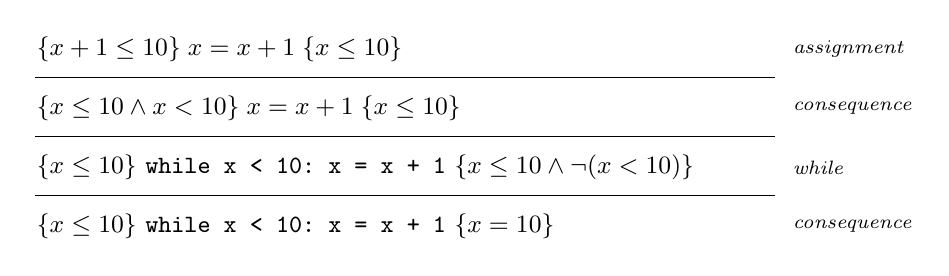
\begin{tikzpicture}[font=\small, t/.style={anchor=west}, rule/.style={font=\scriptsize\itshape, anchor=west}]
  \node[t] at (0, 2.25) {$\{x + 1 \le 10\}\; x = x + 1\; \{x \le 10\}$};
  \node[rule] at (9.6, 2.25) {assignment};
  \draw (0.1, 1.89) -- (9.5, 1.89);
  \node[t] at (0, 1.5) {$\{x \le 10 \wedge x < 10\}\; x = x + 1\; \{x \le 10\}$};
  \node[rule] at (9.6, 1.5) {consequence};
  \draw (0.1, 1.14) -- (9.5, 1.14);
  \node[t] at (0, 0.75) {$\{x \le 10\}$ \texttt{while x < 10:\ x = x + 1} $\{x \le 10 \wedge \neg(x < 10)\}$};
  \node[rule] at (9.6, 0.75) {while};
  \draw (0.1, 0.39) -- (9.5, 0.39);
  \node[t] at (0, 0) {$\{x \le 10\}$ \texttt{while x < 10:\ x = x + 1} $\{x = 10\}$};
  \node[rule] at (9.6, 0) {consequence};
\end{tikzpicture}
\par\smallskip{\small A derivation as a proof tree: each line follows from the one above the bar by the rule named on its right. The two consequence steps need $x \le 10 \wedge x < 10 \Rightarrow x + 1 \le 10$, which holds for 8-bit integers since $x < 10$ rules out the wrap, and $x \le 10 \wedge \neg (x < 10) \Rightarrow x = 10$.}
\end{omfigure}

\omoutput{code/bachelor-3/20-program-verification/outputs/hoare_check.txt}{The derivation of the figure, checked from the leaves up; then a wrong step, rejected with the value that refutes its implication.}\label{out:b3:program-verification:hoare}

\section{Weakest preconditions}\label{sec:b3:program-verification:wp}

\begin{definition}[Weakest precondition, strongest postcondition]\label{def:b3:program-verification:wp}
The \emph{weakest precondition}\index{weakest precondition} $\mathrm{wp}(S, Q)$ is a formula that holds in exactly the states from which every run of $S$ terminates in a state satisfying $Q$. The \emph{strongest postcondition}\index{strongest postcondition} $\mathrm{sp}(P, S)$ holds in exactly the states that runs of $S$ from $P$ can end in.
\end{definition}

For loop-free programs, wp is computed backwards, one statement at a time:
\[
\mathrm{wp}(x = e, Q) = Q[e/x], \quad \mathrm{wp}(S_1; S_2, Q) = \mathrm{wp}(S_1, \mathrm{wp}(S_2, Q)), \quad \mathrm{wp}(\text{\code{assert} } b, Q) = b \wedge Q,
\]
and the \code{if} gives $(b \Rightarrow \mathrm{wp}(S_1, Q)) \wedge (\neg b \Rightarrow \mathrm{wp}(S_2, Q))$; with \code{unknown()} as its test, both branches may run, and wp is the conjunction of the two.

\begin{theorem}[Weakest preconditions decide triples]\label{thm:b3:program-verification:wp}
For a loop-free $S$, $\{P\}\,S\,\{Q\}$ is valid if and only if $P \Rightarrow \mathrm{wp}(S, Q)$ is valid.
\end{theorem}

By induction on $S$, the formula computed holds in a state exactly when every run of $S$ from it ends in $Q$; the triple is then the implication. Edsger Dijkstra introduced \omterm{def:b3:program-verification:wp}{weakest preconditions} in 1975. % ledger: b3:dijkstra-1975

\omcode{code/bachelor-3/20-program-verification/listings/wp.py}{28}{48}{\omterm{def:b3:program-verification:wp}{Weakest preconditions} of loop-free programs.}\label{lst:b3:program-verification:wp}

\omoutput{code/bachelor-3/20-program-verification/outputs/wp.txt}{Three \omterm{def:b3:program-verification:wp}{weakest preconditions}, not simplified: the swap through \texttt{t} exchanges $a$ and $b$ in the postcondition.}\label{out:b3:program-verification:wp}

A loop has no finite formula for its wp in general; it would be the limit of unrolling the loop again and again. The programmer supplies an invariant instead, and the verifier checks it.

\section{Verification conditions handed to a solver}\label{sec:b3:program-verification:vc}

\begin{definition}[Annotated program, verification condition, bit-blasting]\label{def:b3:program-verification:vc}
An \emph{annotated program}\index{annotated program} carries an invariant on every loop, and optionally a variant. Its \emph{verification conditions}\index{verification condition} are formulas without programs, whose validity implies that the program meets its specification. \emph{Bit-blasting}\index{bit-blasting} turns a formula over fixed-width integers into a propositional formula with one variable per bit, adders and comparators being written as Boolean circuits.
\end{definition}

The generator computes wp backwards, but takes a loop's invariant $I$ as its precondition and emits three conditions for it: \emph{preserved}, $I \wedge b \Rightarrow \mathrm{wp}(S, I)$; \emph{exit}, $I \wedge \neg b \Rightarrow Q$; and, with a variant $V$, \emph{variant}, $I \wedge b \wedge V = v_0 \Rightarrow \mathrm{wp}(S, V < v_0)$. A final condition, \emph{entry}, says that the precondition implies what the program needs at its start.

\omcode{code/bachelor-3/20-program-verification/listings/vcgen.py}{16}{40}{The \omterm{def:b3:program-verification:vc}{verification conditions} of an \omterm{def:b3:program-verification:vc}{annotated program}.}\label{lst:b3:program-verification:vcgen}

Each condition $F$ is valid exactly when $\neg F$ is unsatisfiable. The bit-blaster gives each 8-bit variable eight Boolean variables and each operation a circuit: a ripple-carry adder for $+$, the same adder on the complement plus one for $-$, a shift for halving, and the borrow of a subtraction for $<$. Each gate becomes a few clauses (Tseitin's encoding), and CDCL decides the result. A satisfying assignment of $\neg F$ is a counterexample: values of the variables that make the condition false.

\omcode{code/bachelor-3/20-program-verification/listings/bitblast.py}{39}{71}{Words of bits, the adder, and comparison through the borrow.}\label{lst:b3:program-verification:bitblast}

\begin{omfigure}
\begin{tikzpicture}[font=\small, >=Stealth, b/.style={draw, rounded corners, fill=omDef!12, minimum height=8mm, align=center}]
  \node[b] (p) at (0, 0) {annotated\\program};
  \node[b] (v) at (2.6, 0) {verification\\conditions};
  \node[b] (c) at (5.2, 0) {CNF of\\$\neg F$};
  \node[b] (s) at (7.6, 0) {CDCL};
  \node[b, fill=omDef!25] (ok) at (10.2, 0.7) {unsat: valid};
  \node[b, fill=omThm!20] (no) at (10.2, -0.7) {model: counter-\\example};
  \draw[->] (p) -- node[above, font=\scriptsize] {awp} (v);
  \draw[->] (v) -- node[above, font=\scriptsize] {bits} (c);
  \draw[->] (c) -- (s);
  \draw[->] (s) -- (ok);
  \draw[->] (s) -- (no);
\end{tikzpicture}
\par\smallskip{\small The verification pipeline of this section.}
\end{omfigure}

Binary search keeps an interval $[lo, hi)$ of indices and halves it. Its array test is replaced by \code{unknown()}, so the proof below covers every array; the assertion checks that the midpoint is a valid index of the interval, and the variant $hi - lo$ proves termination.

\omcode{code/bachelor-3/20-program-verification/listings/verify_bsearch.py}{9}{21}{Binary search, with \texttt{MID} and \texttt{INV} filled in three ways.}\label{lst:b3:program-verification:bsearch}

\omoutput{code/bachelor-3/20-program-verification/outputs/verify_bsearch.txt}{The midpoint $(lo + hi) // 2$ fails, with a counterexample the program reaches; $lo + (hi - lo) // 2$ is verified; and a wrong invariant is caught at entry ($n = 0$) and when kept.}\label{out:b3:program-verification:bsearch}

With $lo = 128$ and $hi = 192$, $lo + hi = 320$, which wraps to 64 in 8 bits, and the midpoint 32 lies below $lo$. The same failure happens with 32-bit indices on arrays of more than $2^{30}$ elements, and the cure, $lo + (hi - lo)/2$, is the same. % ledger: b3:bsearch-overflow
The interpreter confirms the counterexample is not an artefact of the invariant: run on $n = 255$, always choosing the upper half, the assertion fails at $lo = 128$, $hi = 255$.

\section{Temporal properties}\label{sec:b3:program-verification:temporal}

Programs that run forever, such as operating systems, lifts and protocols, are specified by what must hold along their runs: two lifts are never in the shaft together; every request is eventually served.

\begin{definition}[Kripke structure, temporal logic, computation tree logic, linear temporal logic]\label{def:b3:program-verification:kripke}
A \emph{Kripke structure}\index{Kripke structure} is a finite set of states, a successor relation in which every state has at least one successor, and for each state the set of atomic propositions true in it. A \emph{temporal logic}\index{temporal logic} speaks of the runs, infinite paths of states. \emph{Computation tree logic}\index{computation tree logic} (CTL) pairs a path quantifier, E (some path) or A (all paths), with a temporal operator, X (next state), F (some future state), G (every future state) or U (until): $\mathrm{E}[f \,\mathrm{U}\, g]$ holds when some path reaches a $g$-state through $f$-states. \emph{Linear temporal logic}\index{linear temporal logic} (LTL) has the temporal operators without path quantifiers, and a formula holds in a state when it holds on every path from it.
\end{definition}

Everything is expressed with EX, EU and EG: $\mathrm{EF}\,g = \mathrm{E}[\mathrm{true} \,\mathrm{U}\, g]$, $\mathrm{AG}\,f = \neg \mathrm{EF} \neg f$, $\mathrm{AF}\,f = \neg \mathrm{EG} \neg f$. E. M. Clarke and E. A. Emerson proposed CTL in 1981; Amir Pnueli proposed LTL for program verification in 1977. % ledger: b3:clarke-emerson-1981
% ledger: b3:pnueli-1977

\begin{theorem}[Fixed points of CTL]\label{thm:b3:program-verification:fixpoints}
$\mathrm{E}[f \,\mathrm{U}\, g]$ is the \omterm{def:b3:program-optimisation:lfp}{least fixed point} of $Z \mapsto g \vee (f \wedge \mathrm{EX}\,Z)$, and $\mathrm{EG}\,f$ is the greatest \omterm{def:b3:program-optimisation:lfp}{fixed point} of $Z \mapsto f \wedge \mathrm{EX}\,Z$, sets of states being ordered by inclusion.
\end{theorem}

For EF, the $k$-th iterate from the empty set is the set of states that reach $g$ in fewer than $k$ steps, and the iteration stops after at most as many rounds as there are states (\cref{exo:b3:program-verification:11}). The greatest \omterm{def:b3:program-optimisation:lfp}{fixed point} is computed from the full set downwards. So a CTL formula is checked in time polynomial in the size of the structure, by \code{ctl.py}.

\omcode{code/bachelor-3/20-program-verification/listings/ctl.py}{15}{45}{A CTL model checker: one case per operator, EU and EG by iteration to a \omterm{def:b3:program-optimisation:lfp}{fixed point}.}\label{lst:b3:program-verification:ctl}

\begin{omfigure}
\begin{tikzpicture}[font=\small, >=Stealth, s/.style={circle, draw, minimum size=11mm, align=center, inner sep=1pt}]
  \fill[omDef!12, rounded corners] (-0.9, -2.75) rectangle (4.4, 0.9);
  \node[font=\scriptsize, omDef, anchor=south west] at (-0.85, -2.7) {EF done};
  \node[s] (s0) at (0, 0) {0\\\scriptsize start};
  \node[s] (s1) at (6.2, 0) {1\\\scriptsize busy};
  \node[s] (s2) at (0, -1.6) {2\\\scriptsize busy};
  \node[s, fill=omThm!20] (s3) at (3.3, -1.6) {3\\\scriptsize done};
  \draw[->] (s0) -- (s1);
  \draw[->] (s0) -- (s2);
  \draw[->] (s2) -- (s3);
  \draw[->] (s3) to[bend right=15] (s0.south east);
  \draw[->] (s1) to[loop right] (s1);
  \draw[->] (s3) to[loop right] (s3);
\end{tikzpicture}
\par\smallskip{\small The structure of \cref{out:b3:program-verification:ctl}. The shaded region is EF done; state 1 loops on busy forever, so EG busy holds there, and AF done fails at state 0, whose path to state 1 never reaches done.}
\end{omfigure}

\omoutput{code/bachelor-3/20-program-verification/outputs/ctl.txt}{Formulas on the four-state structure; and on a second structure, the formula AF AG p, which fails where the LTL formula F G p holds.}\label{out:b3:program-verification:ctl}

The two logics differ. In the second structure, state 0 loops on $p$ or moves to state 1 ($\neg p$) and then to state 2, which loops on $p$. Every path eventually stays in $p$ for ever, so the LTL formula F G $p$ holds at state 0. But AF AG $p$ fails there: along the path that stays at state 0, no state satisfies AG $p$, since state 1 is still reachable from each of them. Each logic expresses some properties the other cannot; LTL is not built in this chapter.

\section{Model checking finite-state systems}\label{sec:b3:program-verification:mc}

\begin{definition}[Model checking, counterexample trace, state explosion]\label{def:b3:program-verification:mc}
\emph{Model checking}\index{model checking} decides whether a finite-state system, given as a \omterm{def:b3:program-verification:kripke}{Kripke structure}, satisfies a temporal formula, by exploring its states. When a \omterm{def:b3:concurrency:properties}{safety property} AG $f$ fails, a \emph{counterexample trace}\index{counterexample trace} is a path from the start to a state violating $f$. \emph{State explosion}\index{state explosion} is the growth of the number of reachable states, exponential in the number of components of the system.
\end{definition}

\omterm{def:b3:program-verification:mc}{Model checking} began with the work of Clarke and Emerson and of J. P. Queille and J. Sifakis in the early 1980s; Clarke, Emerson and Sifakis shared the 2007 Turing Award for it. % ledger: b3:queille-sifakis-1982
% ledger: b3:mc-turing-2007
The state of Peterson's algorithm for two processes is the two program counters, the two flags and the turn; a step is one process executing one line. Breadth-first search from the start finds the reachable states and builds the \omterm{def:b3:program-verification:kripke}{Kripke structure}, and \code{ctl.py} checks mutual exclusion, AG $\neg(\mathit{crit}_0 \wedge \mathit{crit}_1)$, and that process 0 can always still reach its critical section, AG EF $\mathit{crit}_0$.

\omcode{code/bachelor-3/20-program-verification/listings/peterson_mc.py}{12}{26}{One step of Peterson's algorithm.}\label{lst:b3:program-verification:peterson}

\omoutput{code/bachelor-3/20-program-verification/outputs/peterson_mc.txt}{Peterson's algorithm has 20 reachable states and keeps mutual exclusion; without the turn, a process that tests the other's flag before raising its own lets both in, and breadth-first search finds a shortest trace, of 4 steps.}\label{out:b3:program-verification:peterson}

Breadth-first search finds shortest counterexamples, the easiest to read: both processes see the other's flag down, then both raise their own and enter. A system of $n$ processes with $k$ states each can have up to $k^n$ states, and the weekend problem measures that growth. Model checkers fight it with symbolic representations of sets of states, and with partial-order reduction, which explores only one order of steps that commute; both are told here, not built.

\section{Exercises}\label{sec:b3:program-verification:exercises}

\begin{exercise}[$\star$]\label{exo:b3:program-verification:1}
Compute $\mathrm{wp}(x = x + y;\; y = x - y;\; x = x - y,\; x = a \wedge y = b)$ by hand, and say what the program does, in 8-bit arithmetic too.
\end{exercise}

\begin{exercise}[$\star$]\label{exo:b3:program-verification:2}
Is $\{x < 200\}\; x = x + 100\; \{x \ge 100\}$ valid with 8-bit unsigned integers? With unbounded integers?
\end{exercise}

\begin{exercise}[$\star$]\label{exo:b3:program-verification:3}
Give an invariant that proves $\{n \le 20\}$ \texttt{s = 0; i = 0; while i < n:\ i = i + 1; s = s + i} $\{2s = n(n + 1)\}$ with unbounded integers. What is the largest $n$ for which the 8-bit loop computes $s$ without wrapping?
\end{exercise}

\begin{exercise}[$\star$]\label{exo:b3:program-verification:4}
States 0 to 3; edges $0 \to 1$, $1 \to 2$, $2 \to 1$, $2 \to 3$, $3 \to 3$; $p$ holds in 1 and 3. Predict what \code{ctl.py} prints for EX $p$, EG $p$, AF $p$ and E[$\neg p$ U $p$].
\end{exercise}

\begin{exercise}[$\star\star$]\label{exo:b3:program-verification:5}
\code{exercises/ex5_vcgen.py} generates \omterm{def:b3:program-verification:vc}{verification conditions} for loops but forgets one. Find a wrong program and postcondition it accepts, say which condition is missing, and fix it.
\end{exercise}

\begin{exercise}[$\star\star$]\label{exo:b3:program-verification:6}
Write \code{for_vcs}, the \omterm{def:b3:program-verification:vc}{verification conditions} of a counted loop \code{for i in range(a, b)} with invariant $I$, from the rule in the file's docstring. It is tested on a counting loop and on a wrong one.
\end{exercise}

\begin{exercise}[$\star\star$]\label{exo:b3:program-verification:7}
Prove the \omterm{def:b3:program-verification:hoare}{assignment axiom} sound: if $Q[e/x]$ holds in state $\sigma$, then $Q$ holds in $\sigma[x \mapsto v]$, where $v$ is the value of $e$ in $\sigma$.
\end{exercise}

\begin{exercise}[$\star\star$]\label{exo:b3:program-verification:8}
Starting from the state $(0, 0, 0, 0, 0)$ of \cref{lst:b3:program-verification:peterson}, list by hand the states reachable in one and in two steps. Which of them have a process blocked?
\end{exercise}

\begin{exercise}[$\star\star$]\label{exo:b3:program-verification:9}
Write ``every request is eventually granted'' in CTL and in LTL, with propositions \textit{req} and \textit{grant}. Is \code{AG EF crit0} of \cref{out:b3:program-verification:peterson} such a property? What does a \omterm{def:b3:concurrency:properties}{liveness property} of Peterson's algorithm need that the model lacks?
\end{exercise}

\begin{exercise}[$\star\star\star$]\label{exo:b3:program-verification:10}
Prove the while rule sound: if every terminating run of $S$ from $I \wedge b$ ends in $I$, then every terminating run of \texttt{while b:\ S} from $I$ ends in $I \wedge \neg b$.
\end{exercise}

\begin{exercise}[$\star\star\star$]\label{exo:b3:program-verification:11}
Prove that EF $g$ is the \omterm{def:b3:program-optimisation:lfp}{least fixed point} of $Z \mapsto g \vee \mathrm{EX}\,Z$, and that iteration from the empty set reaches it in at most $|S|$ rounds.
\end{exercise}

\begin{exercise}[$\star\star\star$]\label{exo:b3:program-verification:12}
Verify insertion sort on four values below 16, unrolled into \omterm{def:b3:concurrency:atomics}{compare-and-swap} steps, by \omterm{def:b3:program-verification:vc}{bit-blasting} the program itself: each variable a word of gates, each \code{if} merged with multiplexers. Prove that the result is sorted and made of the inputs, report the size of the CNF, and break one comparison to see a counterexample. Why not use wp here?
\end{exercise}

\section{Weekend problem}\label{sec:b3:program-verification:problem}

\begin{problem}[{Weekend problem --- Two lifts and one shaft}]\label{pb:b3:program-verification:1}
A lift tower shares one section of shaft between its lifts; at most one lift may be in it. Each lift goes from \emph{idle} to \emph{waiting}, then into the \emph{shaft}, and back to idle, and a lock bit guards the shaft. In the correct protocol a waiting lift takes a free lock in one atomic step; in the buggy one it tests the lock in one step and takes it in the next. The model is in \code{lifts.py}.

\omcode{code/bachelor-3/20-program-verification/listings/lifts.py}{12}{27}{One step of one lift.}\label{lst:b3:program-verification:lifts}

\omoutput{code/bachelor-3/20-program-verification/outputs/lifts.txt}{Reachable states of the correct protocol for 1 to 6 lifts, the length of the shortest run that breaks the buggy one, and a fit of the growth.}\label{out:b3:program-verification:lifts}

\medskip\noindent\textbf{Part I --- The model.}
\begin{enumerate}
  \item What is a state, and how many states are there before asking which are reachable, for $n$ lifts in the correct protocol?
  \item Why is every state's successor set nonempty, as a \omterm{def:b3:program-verification:kripke}{Kripke structure} requires?
  \item List the reachable states for one lift.
  \item Why does interleaving, one lift moving per step, model lifts that run at the same time?
  \item List the 8 reachable states for two lifts.
  \item Which unreachable states does the lock exclude?
\end{enumerate}

\medskip\noindent\textbf{Part II --- The properties.}
\begin{enumerate}[resume]
  \item Write mutual exclusion in CTL for two lifts.
  \item Write ``a waiting lift can always still get in'' in CTL.
  \item Why does ``a waiting lift eventually gets in'', AG(\textit{wait} $\Rightarrow$ AF \textit{shaft}), fail in this model?
  \item What assumption about the scheduler would make it true?
  \item Is mutual exclusion a safety or a \omterm{def:b3:concurrency:properties}{liveness property}, and what does a counterexample to each look like?
  \item Why is AG $f$ checked by reachability alone?
\end{enumerate}

\medskip\noindent\textbf{Part III --- The bug.}
\begin{enumerate}[resume]
  \item Give the 6-step trace that breaks the buggy protocol for two lifts.
  \item Why is it the shortest?
  \item Why is it also 6 steps for 3, 4, 5 and 6 lifts?
  \item Would testing many times before taking the lock fix the bug?
  \item Which instruction of a processor makes the correct protocol's atomic step possible?
  \item Relate the bug to Peterson's variant without turn.
\end{enumerate}

\medskip\noindent\textbf{Part IV --- State explosion.}
\begin{enumerate}[resume]
  \item Prove that the correct protocol has $(n + 2) 2^{n - 1}$ reachable states, and check the table.
  \item What growth rate $b$ does the fit report, and why is it above 2?
  \item How many states for 20 lifts, and for 40?
  \item The search stores each state once. At about 100 bytes per state in Python, what memory do 40 lifts need?
  \item The lifts are identical. How could symmetry reduce the count, and to how many states for $n$ lifts?
  \item Sum up: what is verified, what failed and in how many steps, and how the work grows with $n$.
\end{enumerate}
\end{problem}
